\documentclass[a4paper, 10pt]{article}%тип документа

%Русский язык
\usepackage[T2A]{fontenc} %кодировка
\usepackage[utf8]{inputenc} %кодировка исходного кода
\usepackage[english,russian]{babel} %локализация и переносы

\usepackage{multirow}

%Вставка картинок
\usepackage{cellspace, graphicx, makecell}
\DeclareGraphicsExtensions{.pdf,.png,.jpg}

\renewcommand\cellspacetoplimit{3pt}
\renewcommand\cellspacebottomlimit{3pt}
\newcommand\rowincludegraphics[2][]{\raisebox{-0.45\height}{\includegraphics[#1]{#2}}}

%Производные
\usepackage{physics}

%Математика
\usepackage{amsmath, amsfonts, amssymb, amsthm, mathtools}
\usepackage[left=10mm, top=20mm, right=18mm, bottom=15mm, footskip=10mm]{geometry}

%Заголовок
\author{Дербенев Никита Максимович}
\title{Лабораторная работа 1.4.1\\
	Изучение экспериментальных погрешностей на примере физического маятника}
\date{26 октября 2023}
\begin{document}
	\maketitle
	\paragraph {Цель работы:}
	Измерение момента инерции ряда тел и сравнение результатов с расчетами по теоретическим формулам; проверка аддитивности моментов инерции и справедливости формулы Гюйгенса-Штейнера.
	\paragraph{В работе используются:}
	\begin{enumerate}
		\item Трифилярный подвес
		\item Штангенциркуль
		\item Линейка
		\item Счетчик числа колебаний и периода
		\item Набор тел
	\end{enumerate}
	\paragraph{Ход работы:}
	\begin{enumerate}
		\item Проверим, достаточно хорошо ли выполняется соотношение $T \gg \tau$. Измерим для пустой платформы $\tau$ - время уменьшения амплитуды колебаний в 2 раза для угла $30^\circ, 15^\circ$ и приблизительный период колебаний (табл. 1):
		
		\begin{table}[h]
			\centering
			\caption{Измерения $\tau, T$}
			\begin{tabular}{|c|c|c|}
				\hline
				$\tau_{30}, c$ & $\tau_{15}, c$ & $T, c$ \\
				\hline
				335 & 379 & 4.4 \\
				\hline
			\end{tabular}
		\end{table}
		Видно, что результаты отличатся более, чем в 70 раз, следовательно делаем вывод, что соотношение выполняется хорошо и потери в системе достаточно маленькие.
		\item Найдем рабочий диапазон амптитуд колебаний. Для этого будем уменьшать амплитуду колебаний до тех пор, пока период колебаний не перестанет зависеть от амплитуды. Измерим период и занесем в табл. 2:
		
		\begin{table}[h]
			\centering
			\caption{Измерения амплитуды}
			\begin{tabular}{|l|c|c|c|c|c|}
				\hline
				$\varphi$ & $30^\circ$ & $15^\circ$ & $10^\circ$ & $7^\circ$ & $5^\circ$ \\
				\hline
				$T, c$ & 4.48 & 4.39 & 4.37 & 4.36 & 4.36 \\
				\hline
			\end{tabular}
		\end{table}
		
		Как видим, период колебаний перестает изменяться при $\varphi = 7^\circ$, значит можно использовать его для дальнейших измерений. Использовать меньший угол не имеет смысла, так как точность измерений от этого не увеличивается, а сложность измерений возрастает.
		
		\item Определим необходимое количество колебаний для измерений периода с точностью $\varepsilon_T = 0.5\%$.
		\[N = \dfrac{\sigma_T}{T\varepsilon_T} < 1\]
		Для надежности возьмем $N = 5$, так как кроме систематической, измерения могут содержать случайную погрешность (особенности счетчика).

		\item Измерим параметры установки $l$, $R$ и $r$, $m$ их погрешности (табл.3). Найдем $z_0$ по формуле:
		\[z_0 = \sqrt{l^2 - R^2} = \sqrt{2154^2 - 114.6^2} = (2151 \pm 2) \text{ мм}\]
		
		\begin{table}[h]
			\centering
			\caption{Параметры установки}
			\begin{tabular}{|l|c|c|c|}
				\hline
				& Величина & $\sigma$ & $\varepsilon$ \\
				\hline
				$l$, мм & 2154.0 & 2 & 0.0009 \\
				\hline
				$z_0$, мм & 2151.0 & 2 & 0.0009 \\
				\hline
				$r$, мм & 30.5 & 0.3 & 0.0098 \\
				\hline
				$R$, мм & 114.6 & 0.5 & 0.0004 \\
				\hline
				$m$, г & 934.7 & 0.5 & 0.0005 \\
				\hline
			\end{tabular}
		\end{table}
		
		Вычислим константу $k$ для данной установки и ее погрешность:
		\[k = \dfrac{gRr}{4\pi^2z_0} \approx 0.404 \cdot 10^{-3} \frac{\text{м}^2}{c^2}\]
		\[\varepsilon_k = \varepsilon_g + \varepsilon_R + \varepsilon_r + \varepsilon_{z_0} \approx 0.0111\]
		\[\sigma_k = k\varepsilon_k \approx 0.037 \cdot 10^{-3} \frac{\text{м}^2}{c^2}\]
		
		\[k = \left(0.40 \pm 0.04\right) \cdot 10^{-3} \frac{\text{м}^2}{c^2}\]
		
		\item Опрелелим момент инерции ненагруженной платформы $I_0$:
		\[I_0 = kmT^2 \approx 7.11 \cdot 10^{-3} \text{ кг}\cdot\text{м}^2\]
		\[\varepsilon_{I_0} = \varepsilon_k + \varepsilon_m + 2\varepsilon_T \approx 0.0216\]
		\[\sigma_{I_0} = I_0\varepsilon_{I_0} \approx 0.154 \cdot 10^{-3} \text{ кг}\cdot\text{м}^2\]
		
		\[I_0 = (7.11 \pm 0.15) \cdot 10^{-3} \text{ кг}\cdot\text{м}^2\]
		
		\item Измерим параметры имеющихся тел:
		
		\begin{table}[h]
			\centering
			\caption{Параметры тел}
			\begin{tabular}{|c|c|c|c|c|c|c|}
				\hline
				№ & Схема & Параметры & T, c & $I + I_0, 10^{-3} \text{ кг}\cdot\text{м}^2$ & $I, 10^{-3} \text{ кг}\cdot\text{м}^2$ & $I_\text{теор}, 10^{-3} \text{ кг}\cdot\text{м}^2$\\
				\hline
				1 & \rowincludegraphics{body1} &
				\begin{tabular}{c}
					$h = (55.4 \pm 0.1) \text{ мм}$ \\
					$d = (3.9 \pm 0.1) \text{ мм}$ \\
					$D = (158.5 \pm 0.1) \text{ мм}$ \\
					$m$ = 748.0 г \\
				\end{tabular} & 4.150 & 11.59 & $4.48 \pm 0.25$ & 4.58 \\
				\hline
				2 & \rowincludegraphics{body2} &
				\begin{tabular}{c}
					$a = (26.9 \pm 0.1) \text{ мм}$ \\
					$b = (26.9 \pm 0.1) \text{ мм}$ \\
					$c = (208.5 \pm 0.1) \text{ мм}$ \\
					$m$ = 1177.5 г \\
				\end{tabular} & 3.69 & 11.56 & $4.45 \pm 0.25$ & 4.33 \\
				\hline
				3 & \rowincludegraphics{body3} &
				\begin{tabular}{c}
					$d = (20.0 \pm 0.1) \text{ мм}$ \\
					$D = (158.5 \pm 0.1) \text{ мм}$ \\
					$h = (7.0 \pm 0.1) \text{ мм}$ \\
					$H = (30.5 \pm 0.1) \text{ мм}$ \\
					$m$ = 1122.9 г \\
				\end{tabular} & 3.584 & 10.57 & $3.46 \pm 0.23$ & 3.30\\
				\hline
				1 + 3 & & m = 1870.9 г & 3.664 & 15.07 & $7.96 \pm 0.33$ & 7.88 \\
				\hline
			\end{tabular}
		\end{table}
		
		Расчитаем теоретические значения моментов инерции тел и запишем в табл. 4:
		\[I_1 = \frac{1}{2}m\left(r_1^2+r_2^2\right) = \frac{1}{2}m\left(\left(\frac{D - d}{2}\right)^2 + \left(\frac{D}{2}\right)^2\right) = 4.58 \cdot 10^{-3} \text{ кг}\cdot\text{м}^2\]
		\[I_2 = \frac{1}{12}m\left(a^2+c^2\right) =  4.33 \cdot 10^{-3} \text{ кг}\cdot\text{м}^2\]
		\newpage
		\[m_1 = m\dfrac{V_1}{V} = m\dfrac{d^2H}{d^2H+D^2h}\]
		\[m_2 = m\dfrac{V_2}{V} = m\dfrac{D^2h}{d^2H+D^2h}\]
		\[I_3 = \frac{1}{8}m_1d^2 + \frac{1}{8}m_2D^2 = \dfrac{1}{8}m\dfrac{d^4H + D^4h}{d^2H+D^2h} = 3.30 \cdot 10^{-3} \text{ кг}\cdot\text{м}^2\] 
		\item Измерим моменты инерций всех тел и запишем в табл. 4. Момент инерции и его погрешность расчитаем по формуле:
		\[I = k(m_0+m)T^2 - I_0\]
		\[\sigma_I = \sigma_{I_0} + \sigma_{I} = \varepsilon_{I_0}I_0 + \varepsilon_{I_0}I = \varepsilon_{I_0} (I_0 + I)\]
		
		Как видим, все измеренные моменты инерции $I_i$ не выходят за пределы погрешности $\sigma_{I_i}$.
		
		\item Измерим момент инерции тел 1 и 3 вместе, результаты запишем в табл. 4. Как видно из таблицы, аддитивность моментов инерции соблюдается, значение лежит в пределе допустимой погрешности:
		\[I_{1+3} = (7.96 \pm 0.33) \cdot 10^{-3} \text{ кг}\cdot\text{м}^2\]
		\[I_1 + I_3 = (7.94 \pm 0.48) \cdot 10^{-3} \text{ кг}\cdot\text{м}^2\]
		
		\item Поместим на платформу диск, разрезанный по диаметру, горизонтально. Постепенно раздвигая половинки диска так, чтобы их общий центр масс все время оставался на оси вращения платформы, снимем зависимость момента инерции системы $I$ от расстояния $h$ каждой из половинок до центра платформы. Масса грузиков $m$ = 1.336 кг. Расчитаем моменты инерции по формуле и запишем в табл. 5:
		\[I = k(m+m_0)T^2 - I_0\]
		\begin{table}[h]
			\centering
			\caption{Сдвиг половинок цилиндра}
			\begin{tabular}{|c|c||c|c||c|c|c|}
				\hline
				№ & $h$, мм & $T$, c & $I, 10^{-3} \text{ кг}\cdot\text{м}^2$ & $T$, c & $I, 10^{-3} \text{ кг}\cdot\text{м}^2$ \\
				\hline
				1  & 0  & 3.094 & 1.58 & 3.012 & 1.13 \\
				2  & 5  & 3.098 & 1.61 & 3.020 & 1.17 \\
				3  & 10 & 3.116 & 1.71 & 3.040 & 1.29 \\
				4  & 15 & 3.142 & 1.86 & 3.068 & 1.44 \\
				5  & 20 & 3.188 & 2.12 & 3.104 & 1.64 \\
				6  & 25 & 3.226 & 2.34 & 3.164 & 1.98 \\
				7  & 30 & 3.294 & 2.75 & 3.222 & 2.32 \\
				8  & 35 & 3.370 & 3.21 & 3.298 & 2.77 \\
				9  & 40 & 3.444 & 3.66 & 3.382 & 3.28 \\
				10 & 45 & 3.550 & 4.34 & 3.466 & 3.80 \\
				11 & 50 & 3.634 & 4.88 & 3.562 & 4.41 \\
				\hline
			\end{tabular}
		\end{table}
		
		Построим график зависимости $I(h^2)$. По графику видно, что он представляет собой линейную зависимость $I = kh^2 + b$.
		
		По формуле Гюйгенса-Штейнера:
		
		\[I(h) = I + mh^2\]
		
		Найдем коэффициенты по МНК:
		
		\[I = b = (1.565 \pm 0.009) \cdot 10^{-3} \text{ кг}\cdot\text{м}^2\]
		\[m = k = (1.335 \pm 0.011) \text{ кг}\]
		
		\item Повторим измерения для вертикального положения половинок, запишем в табл. 5.
		
		\begin{figure}[h]
			\centering
			\caption{Графики зависимостей $I(h^2)$ для разных положений половинок}
			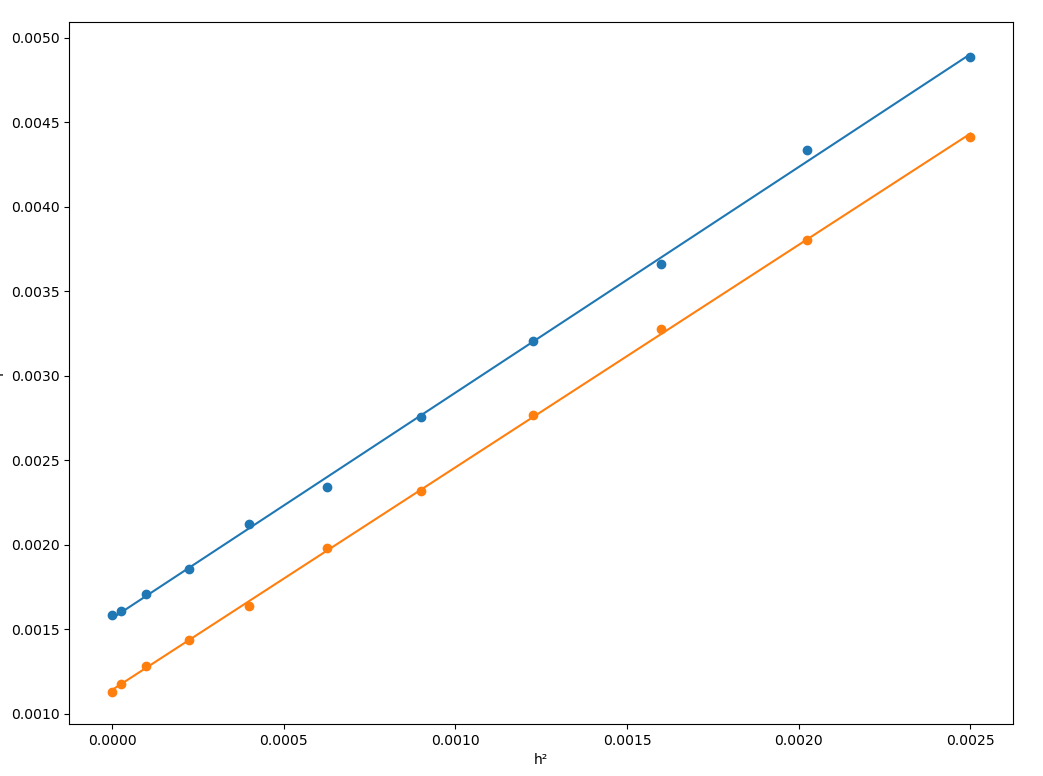
\includegraphics{graph}
		\end{figure}
		
		Найдем коэффициенты по МНК:
		
		\[I = b = (1.142 \pm 0.005) \cdot 10^{-3} \text{ кг}\cdot\text{м}^2\]
		\[m = k = (1.336 \pm 0.006) \text{ кг}\]
		
		Как видно из эксперимента, формула Гюйгенса-Штейнера работает, а массы цилиндра, вычисленные по МНК, лежат в пределах допустимой погрешности.
		
		\paragraph{Вывод}
		С помощью трифилярного подвеса можно определять момент инерции с достаточно большой точностью $\varepsilon_{I_0} \approx 2.2\%$. Такая точность обусловлена малой погрешностью измерения времени и условиями, при которых колебания подвеса можно считать слабозатухающими.
		
		Мы экспериментально доказали аддитивность моментов инерции с помощью различных тел.
		
		Полученная зависимость $I(h^2)$ аппроксимируется линейной зависимостью, что подвтерждает формулу Гюйгенса-Штейнера ($I = I_c + Mh^2$, где $I$ -- момент инерции тела, $I_c$ --момент инерции тела относительно центра, $M$ -- масса тела, а $h$ -- расстояние между двумя осями, в нашем случае -- между осью вращения и половинками диска).
		
		
	\end{enumerate}
\end{document}